\documentclass[twocolumn]{article}

\usepackage{mathtools}
\usepackage{amsmath,amsfonts}
\usepackage{lscape}
\usepackage{bm}
\usepackage{breqn}
\usepackage{hyperref}
\usepackage{rotating}
\usepackage{pseudocode}

\usepackage{graphicx}
\usepackage[utf8]{inputenc}

\usepackage{tikz}
\usetikzlibrary{shapes.geometric,calc}
\usetikzlibrary{patterns}

\usepackage[square,sort,comma,numbers]{natbib}

\tikzset{
	pro/.style={circle,draw=black,fill=none,inner sep=1pt,minimum size=1.3em},
	sil/.style={circle,draw=none,fill=black,inner sep=0pt,minimum size=5pt}
}

\DeclareBoldMathCommand{\t}{t}
\DeclareMathOperator{\loss}{\ell}
\newcommand{\segs}{\mathbb S}
\newcommand{\head}{\mathcal H}
\newcommand{\tail}{\mathcal T}
\newcommand{\best}{\mathcal V}

\usepackage{multirow}
\usepackage{array}
\usepackage{colortbl}

\newlength\epaisLigne
\newcommand\Mline[2]{\noalign{\global\epaisLigne\arrayrulewidth\global\arrayrulewidth#1pt}\cline{#2}\noalign{\global\arrayrulewidth\epaisLigne}}

%\newcommand{\mynote}[1]{\marginpar{\tiny #1}}
\newcommand{\mynote}[1]{}

\hypersetup{
	pdfauthor={Tim Scarfe, Wouter M. Koolen and Yuri Kalnishkan},
	pdftitle={Segmenting electronic dance music streams based on self-similarity},
	pdfkeywords={audio,stream,segmentation,dj,mixing},
	pdfsubject={Artificial Intelligence},
	pdfcreator={Tim Scarfe},
	pdfproducer={Tim Scarfe},
}
\title{
	A long-range self-similarity approach to segmenting DJ mixed music streams}
\author{Tim Scarfe, Wouter M.~Koolen and Yuri Kalnishkan \\ 
	Computer Learning Research
	Centre and Department of Computer Science, \\ 
	Royal Holloway,  University of London, Egham, Surrey, TW20 0EX, United Kingdom\\
	\{tim,wouter,yura\}@cs.rhul.ac.uk
}

\pagestyle{plain}
% to remove in the final version!!


%\renewcommand*{\algorithmcfname}{Protocol}
% see http://tex.stackexchange.com/questions/22477/renaming-algorithm-to-heuristic-in-algorithm2e-package


\title{Segmenting electronic dance music streams based on self-similarity}
\begin{document}
	
	\maketitle
	
	\begin{abstract}
		
		We describe an unsupervised, deterministic algorithm for segmenting DJ-mixed Electronic Dance Music (EDM) streams (for example; pod-casts, radio shows, live events) into their respective tracks. We attempt to reconstruct boundaries as close as possible to what a human domain expert would create in respect of the same task. The goal of DJ-mixing is to render track boundaries effectively invisible from the standpoint of human perception which makes the problem difficult.
		
		We use dynamic programming to optimally segment a cost matrix derived from a self-similarity matrix. The similarity matrix is based on the cosines of a time series of kernel-transformed Fourier based features. Our method is applied to EDM streams. Its formulation incorporates long-term self similarity as a first class concept combined with dynamic programming and it is qualitatively assessed on a large corpus of long streams that have been labelled by a domain expert.
		\smallskip
		
		\noindent \textbf{Keywords.} \noindent music,segmentation,DJ mix,dynamic programming
		
	\end{abstract}
	
	
	\vspace{1em}
	
	\section{Introduction}
	
	Electronic Dance Music tracks are usually mixed by a disc jockey (DJ). For this reason EDM music streams are quite unique compared to other genres of music. Mixing is the \textit{modus operandi} in electronic music. We first transform the audio file into a time series of features discretized into adjacent tiles and transform them into a domain where some pairs from the same track would be distinguishable by their cosine. Our features are based on a Fourier transform with convolution filtering to accentuate prominent instruments and self-similarity within tracks. We create a similarity matrix from these cosines and then derive cost matrices showing the costs of fitting a track at a given time with a given length. We use Dynamic Programming (DP) to create the cost matrix and again to perform the most economical segmentation of the cost matrix to fit a predetermined number of tracks.
	
	A distinguishing feature of our algorithm is that it focuses on long term self similarity of segments rather than transients or a novelty function. Dance music tracks have the property that they are made up of repeating regions, and the ends are almost always similar to the beginning. For this reason we believe that some techniques from structural analysis fail to perform as well for this segmentation task because we focus on the concept of self-similarity ranging over a configurable time horizon. Our method does not require any training or tenuous heuristics to perform well. 
	
	The purpose of this algorithm is to reconstruct optimal boundaries given a fixed number of tracks known in advance (their names and order are known). This is relevant when one has recorded a show, downloaded a track list and needs to reconstruct the indices given a track list. The order of the indices reconstructed is critical so that we can align the correct track names with the reconstructed indices. If the track list was not known in advance the number of tracks could be estimated quite reliably as the variable of track lengths is Gaussian (see Figure~\ref{fig:tracklengths}).
	
	One of the interesting features of audio is that you \textit{can not scrub through it and get an overview in the same way you can with video}. Audio has a reduced \textit{contextual continuum} when the user skips through it perhaps due to the lack of redundant, persistent scene-setting information or indeed a psychological reason. Even in video applications, discovery, context and scrubbing is an active area of research \cite{Matejka:2013:SIO:2470654.2466149}. Time index metadata would allow click through monetisation, and allow improved use-case scenarios (for example publishing track names to social networks, information discovery and retrieval). Capturing metadata in audio is a time consuming and error-prone process. Tzanetakis found in \cite{tzanetakis1999framework} that it took users on average $2$ hours to segment $10$ minutes of audio using standard tools. While not directly relevant we might glean from those findings that there is a strong motivation to automate this process. We have also noticed that while the error variable of the human captured time metadata that we were supplied with appears Gaussian, there is a noticeable deteriorate towards the end of the shows or in relation to the complexity of the mixing by the disc jockey. 
	
	To mix tracks DJs always match the speed or \textit{BPM} (beats per minute) of each adjacent track during a transition and align the major percussive elements in the time domain. This is the central concept of removing any dissonance from overlapping tracks. Tracks can overlap by any amount. DJs increase adjacent track compatibility further by selecting adjacent pairs that are harmonically compatible and by applying spectral transformations (EQ).
	
	The main theme of the early literature was attempting to generate a novelty function to find points of change using distance-based metrics or statistical methods. Heuristic methods with hard decision boundaries were used to find the best peaks. A distinguishing feature of our approach is that we evaluate how well we are doing compared to humans for the same task. We compare our reconstructed indices to the ones created by a human domain expert. 
	
	J.\ Foote et al \citep{foote1999visualizing,foote1997similarity,foote2000automatic,foote2003media,foote2001visualizing} have done a significant amount of work in this area and the first to use similarity matrices. Foote evaluated a Gaussian tapered checkerboard kernel along the diagonal of a similarity matrix to create a 1d novelty function. One benefit to our approach is that our DP allows any range of long-term self similarity (which relates to the fixed kernel size in Foote's work).
	
	Goodwin et al.\ also used DP for segmentation \citep{goodwin2003audio,goodwin2004dynamic}. Their intriguing supervised approach was to perform Linear Discriminant Analysis (LDA) on the features to transform them into a domain where segmentation boundaries would be emphasised and the feature weights normalised. They then reformulated the problem into a clustering DP to find an arbitrary number of clusters. We believe the frame of mind for this work was structural analysis, because it focuses on short term transients (mitigated slightly by the LDA) and would find segments between two regions of long term self similarity. Goodwin was the first to discuss the shortcomings of novelty peak finding approaches. Goodwin's approach is not optimized to work for a predetermined number of segments and depends on the parametrization and training of the LDA transform. 
	
	Peeters et al \citep{peeters2002toward,peeters2004deriving} did some interesting work combining k-means and a transformation of the segmentation problem into Viterbi (a dynamic program).
	
	We compare our error to the relative error of cue sheets created by human domain experts. We focus directly on DJ mixed electronic dance music.
	
	In the coming sections we will describe TODO
	
	\section{Corpus}\label{dataset}
	
	We have been supplied with several broadcasts from three popular radio shows. These are: Magic Island, by Roger Shah ($106$ shows); A State of Trance with Armin Van Buuren ($110$ shows); and Trance Around The World with Above and Beyond ($88$ shows) (Total $304$ shows). The show genres are a mix of Progressive Trance, Uplifting Trance and Tech-Trance. We believe this corpus is the largest of its kind used \cite{peiszer2008automatic} in the literature.  
	The music remains uninterrupted after the introduction (no silent gaps). 
	The shows come in $44100$ samples per second, $16$ bit stereo MP3 files sampled at $192$Kbs. We resampled these to $4000$Hz $16$ bit mono (left+right channel) WAV files to allow us to process them faster. We have used the ``Sound eXchange''\footnote{\url{http://sox.sourceforge.net}}  program to do this. These shows are all $2$ hours long. The overall average track length is $5$ and a half minutes (slightly less for Magic Island) and normally distributed. The average number of tracks is $23$ for ASOT and TATW, $19$ for Magic Island. There is a guest mix on the second half of each show. The guest mix DJs show off their skills with technically convoluted mixing.
	
	\begin{figure}
		\centering
		\includegraphics[width=0.45\textwidth]{images/tracklength.pdf}
		
		\caption{The track length distribution for all three radio shows. The \textit{bump} of short tracks (less than $3$ minutes) are often introductions or otherwise extraneous.}
		\label{fig:tracklengths}
	\end{figure} 
	
	There is already a large community of people interested in getting track metadata for DJ sets. ``CueNation''\footnote{\url{http://www.cuenation.com}} is an example of this. CueNation is a website allowing people to submit \textit{cue sheets} for popular DJ Mixes and radio shows. A cue sheet is a text file containing time metadata (indices) for a media file.
	
	We had our time metadata (indices) and radio shows provided to us and hand captured by \textit{Dennis Goncharov}; a domain expert and one of the principal contributors to \textit{CueNation}. One of the significant problems with this task is that there is an (apparently Gaussian) error variable attached to the human captured indices themselves. On some tracks, it is unclear where to place the optimal index and when analysing our results, we have noticed some obvious human errors. Regrettably, there is no obvious way of quantifying this. Many of the cue sheet authors themselves reject the idea of automating the task citing the poor precision of any such result (they often place indices on the exact MP3 frame). However this sentiment seems misplaced given that they make blatant mistakes or that it is a matter of opinion where to place the track and some consistent method may be preferential. A potential outcome of our method would be a way to assist them with initial placements. Our results demonstrate that it is indeed possible to automate this task and that while there is some uncertainty attached to the optimal placement, it is still largely predictable.
	
	\textit{Dennis Goncharov} provided us with the following description of how he captures the indices. To quote from a personal email exchange with Dennis:
	
	\begin{quote}
		The transition length is usually in factors of $8$ bars ($1$ bar is $4$ beats. At $135$ beats per minute, $8$ bars is $14.2$ sec). It is a matter of personal preference which point of the transition to call the index. My preference is to consider the index to be the point at which the second track becomes the focus of attention and the first track is sent to the background. Most of the time the index is the point at which the bass line ($400$Hz and lower) of the previous track is cut and the bass line of the second track is introduced. If the DJ decides to exchange the adjacent tracks gradually over the time instead of mixing them abruptly then it is up to the cue sheet maker to listen further into the second track noting the musical qualities of both tracks and then go back and choose at which point the second track actually becomes the focus of attention.
	\end{quote}
	
	The most obvious and pervasive element in dance music is the percussion (the beats). We believe on balance that ignoring the percussive information is advantageous, because DJs use percussion primarily to blur boundaries between tracks.  We tried to capture percussive based features and found that the transitions between tracks and indeed groups of tracks appeared as stronger self-similar regions in $S$ than the actual tracks. It is clear from our research that it is the boundaries between instruments and harmonic content that reveals track boundaries, not percussion or rhythm. When we tried implementing a rhythm feature extractor by looking at a transformed autocorrelation of the time domain tiles, it was ineffective because it is the rhythm more than the instruments that is matched between adjacent tracks by the DJs. Some DJs do mix harmonically too but this preys on human hearing and perception. An algorithm capturing the harmonic information would most likely be able to easily distinguish two harmonically compatible tracks. Perhaps more sophisticated rhythm detection (than what we tried) might still work and should be explored further. 
	
	
	\section{Evaluation Criteria}\label{eval_crit}
	
	It is challenging to quantify the performance of our method because if we misplace any tracks, it may have a cascade effect. For example if we place one track too many early on in a show, many of the subsequent tracks may be correctly detected but placed out of alignment. 
	
	We perform three types of evaluation: `\textit{average}', \textit{heuristic precision}', and `\textit{thresholds}'.
	
	The \textit{average} (in seconds) given as $$\frac{1}{|P|}\sum_{i=1}^{|P|}{|P_i-A_i|}$$ is quite simply the mean absolute difference between constructed and actual indices ($P$ is constructed indices, and $A$ is the human indices). Naturally this metric will have a reduced meaning in some sense because although it depends on the real accuracy it also depends on the amount of misplacements and where in the track those misplacements were. The uncertainty variable attached to the misplacements is wide (in relation to the size of the shows and the number of tracks) but does regularise over the course of a large dataset. This metric is the most meaningful for capturing the overall \textit{robustness} of the method.
	
	The \textit{heuristic precision} metric denoted by 
	\[
	\hat H(P,A) =  \mathrm{Median}\left(    \mathrm{Sort}\left( |P-A_i|\right)_1 \right)
	\] for all
	takes the median of the absolute differences between each prediction in $P$ and the nearest actual index in $A$. This is the most meaningful single metric of accuracy, it is largely invariant to misplacements.
	
	The thresholds metric is the percentage of matched tracks within different intervals of time $\{60, 30, 20, 10, 5, 3, 1\}$, in \emph{seconds} as a margin around any of the track indices we have been given. This metric is also invariant to alignment and is provided for comparison with our other paper \cite{scarfe2013long}.
	
	Note that our results will contain the mean average of these metrics (captured for each show) across the dataset being evaluated. 
	
	\section{Preprocessing}\label{proprocessing} % Fourier/xcorr
	
	The dataset had some outliers that may have slightly distorted the analysis of our method. Many of the ``tracks'' in our data set (of indices) were in fact not tracks at all but rather introductions or voice-overs. Almost all of these outlier tracks were short in length. These are quite clearly visible on the distribution of track lengths on Figure~\ref{fig:tracklengths}. To ameliorate the situation we simply removed any tracks that were shorter than $180$ seconds. We also removed any end tracks that were shorter than $240$ seconds as very often the end tracks on a radio show contain some strange elements (for example voice-overs, interviews, show-related `jingles'). This required some manipulation of the cue sheets and audio files. The offending segments of the audio files are chopped out, and the cue sheets are re-flowed so that the time indices point to the correct location in the file. 
	
	The algorithm still performs similarly when removing just these indices and leaving the audio intact underneath, so it would not significantly effect any real-world implementation. 
	
	For those wishing to use this algorithm in practice with pre-recorded shows; the introductions at the start of the shows can be thought of as being fixed length (with a different length for each show type).
	
	\section{Feature Extraction}\label{feat_ex} % Fourier/xcorr
	
	We used SoX (see Sect.~\ref{dataset}) to downsample the shows to $4000$Hz. We are not particularly interested in frequencies above around $2000$Hz because instrument harmonics become less visible in the spectrum as the frequency increases. The Nyquist theorem \cite{nyquist1928certain} states that the highest representable frequency is half the sampling rate, so this explains our reason to use $4000$Hz. We will refer to the sample rate as $R$. Let $L$ be the length of the show in samples.
	
	Fourier analysis allows one to represent a time domain process as a set of integer oscillations of trigonometric functions. We used the discrete Fourier transform (DFT) to transform the tiles into the frequency domain. The DFT 
	$$F(x_k) = X_k = \sum_{n=0}^{N-1} x_n \cdot e^{-i 2 \pi \frac{k}{N} n}$$ transforms a sequence of complex numbers $x_0,\ldots,x_N$ into another sequence of complex numbers $X_0,\ldots,X_N$ where $$e^{-i 2 \pi \frac{k}{N} n}$$ are points on the complex unit circle. Note that the fftw algorithm \cite{frigo2004fftw} that we used to perform this computation operates significantly faster when N is a power of 2 so we zero pad the input to make that the case. Because we are passing real values into the DFT fuction, the second half of the result is a rotational copy of the first half. As we are not always interested in the entire range of the spectrum, we use $l$ to represent a low pass filter (in Hz) and $h$ the high pass filter (in Hz). So we will capture the range from $h$ to $l$ on the first half of the result of $F$. We take the absolute values of the complex DFT result (defined as its distance in the complex plane from the origin using the Pythagorean theorem).
	
	Show samples are collated into a time series $Q_i, i \in \{1,2,\ldots,\lfloor\frac{L}{M_s}\rfloor\} $ of contiguous, non-overlapping, adjacent \emph{tiles} of equal size. Samples at the end of the show that do not fill a complete tile get discarded. We denote the tile width by $M$ in seconds (an algorithm parameter) and $M_s$ in samples $(M_s = M \times R)$. For each tile $t_i \in Q$ we take the DFT $F(t_i)$ and place a segment of it into feature matrix $D_i$ ($|Q|$ feature vectors in $D$). For each DFT transform we select vector elements $\lceil h \times \frac{M_s}{R} \rceil+1$ to $\lceil l \times \frac{M_s}{R} \rceil+1$ to enable spectral filtering.
	
	To focus on the instruments and improve performance we perform convolution filtering on the feature vectors in $D$, using a Gaussian first derivative filter. This works like an edge detection filter but also expands the width of the transients (instrument harmonics) to ensure that feature vectors from the same song appear similar because their harmonics are aligned on any distance measure (we use the cosines). This is an issue because of the extremely high frequency resolution we have from having such large DFT inputs. For example with a tile size of $10$ seconds and a sample rate of $4000$ we have a have a frequency resolution of $\frac{1}{2}10 \cdot 4000 = 20$KHz. Typically a STFT approach is used which has smaller DFTs (for example \cite{tzanetakis1999multifeature}). 
	
	The Gaussian first derivative filter is defined as 
	$$- \frac{2 G}{B^2}  e^{-\frac{G^2}{B^2}} $$ where 
	
	$$G=\left\{-\lfloor 2B\rfloor,\lfloor-2B+1\rfloor,\ldots, \lfloor 2 B \rfloor\right\},$$ and $$B = b \left( \frac{N}{R} \right).$$ $b$ is the bandwidth of the filter in Hz and this is a parameter of the algorithm. After the convolution filter is applied to each feature vector in $D$, we take the absolute values and normalize on the vector lengths.  
	
	Because the application domain is well defined in this setting, we can design features that look specifically for what we are interested in (musical instruments). Typically in the literature; algorithms use an amalgam of general purpose feature extractors. For example; spectral centroid, spectral moments, pitch, harmonicity \cite{tzanetakis1999framework}. We construct a disimilarity matrix of cosines $S ~=~ \left< D_{i} \cdot D_{j} \right>$, center it around the mean $S = S^{2 \cdot \frac{1}{T^2}\sum S_{ij}}$, normalize it by $\hat c$, $S=S^{\hat c}$ then place it on a small interval around $0$. $S_{ij} = \left( 2 \cdot S_{ij} \right)-1$. It is necessary to have \textit{incentives} and \textit{disincentives} for meaningful track placement which is why we opted for this interval. The distribution of values in $S$ is normal with a raised section on left (negatives) representing the tracks we want to find. When $\hat c$ is $1$ there is no change, smaller values will shift the mean below $0$ and vice versa. This will become relevant when we discuss cost matrices as some of them depend on the sign of the value in $S$. 
	
	See Figure~\ref{fig:simmatrix} for an illustration of $S$.
	
	\begin{figure*}[t]
		\centering
		%\includegraphics[width=0.45\textwidth]{simmat_preds1.pdf}
		%\hspace{1em}
		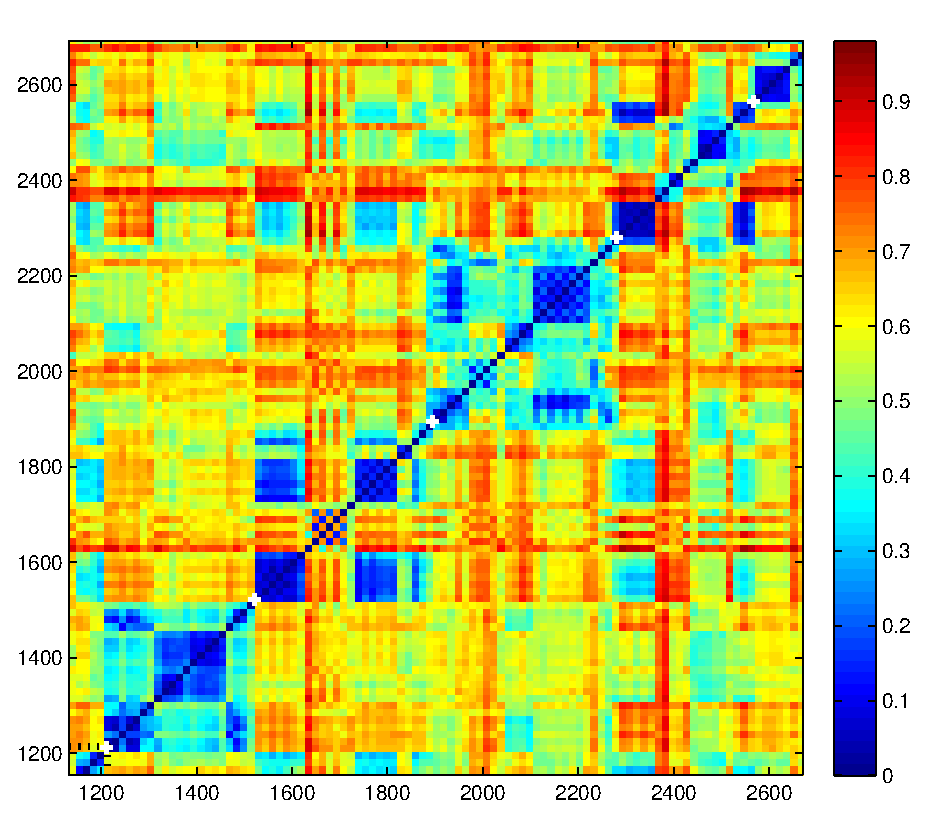
\includegraphics[width=0.4\textwidth]{images/simmat_plain}
		
		\caption{An illustration of the similarity matrix $S$}
		\label{fig:simmatrix}
	\end{figure*} 
	
	\section{Cost Matrices}\label{costmatrix_sec} % dynamic recursion
	
	We now have a similarity matrix $S(i,j)$ as described in Section~\ref{feat_ex}. 
	
	Let $w$ and $W$ denote the minimum and maximum track length in seconds, these will be parameters.
	
	We require a cost matrix $C(f,t)$ that describes the cost of placing a track of length $t-f+1$ at $f$. After analysing the data set, we have created $8$ cost matrices that exploit observed phenomena in $S$. We also provide an additional cost matrix which is just a Gaussian random function centred around the mean track length for all times which can be used to regularise the other $8$ matrices or used on its own as a comparator to a more naive method of placement. 
	
	The more sophisticated matrices exploit themes such as contiguity, symmetry, evolution and change as well as simple summation of $S$ as was presented in our last paper. In our previous work \cite{scarfe2013long} $S$ was on the interval $[0,1]$ and the summation method could only consider disincentives. All of the new matrices have a parameter to shift the consideration of incentive verses disincentive and will contain values on the interval $[-1,1]$.
	
	Intuitively, most tiles within the same track are similar, while pairs of tiles that do not belong to the same track are significantly more dissimilar. However, often this is not the case and many tracks have dissimilar regions within them. 
	
	\subsection{Normalization}
	
	We define $N(C,\Omega)$ as a normalization function for cost matrix $C$ and incentive bias $\Omega$. It will return a $[-1,1]$ interval when $\Omega=0.5$, $[-1,0]$ when $\Omega=1$  and $[0, 1]$ when $\Omega=0$ and will produce a convex interpolation for other values.
	
	Let 
	\begin{dmath*}
		\hat N(C,\Omega) = \left( \frac{ C_{ij} - \min \left( C_{ij} \right) }{ \max \left( C_{ij} \right) - \min \left( C_{ij} \right) } \cdot \hat h  \right)-s
	\end{dmath*}
	for all $i,j \in C$ where $\hat h$ = $2-\left( 2\cdot|0.5-\Omega| \right)$ and 
	\begin{dmath*}
		s= { \left\{
			\begin{array}{ll}
				\Omega > 0.5  & :   1-2 \cdot |0.5-\Omega|  \\
				\Omega <= 0.5 & : 1.  \\
			\end{array}
			\right.}
	\end{dmath*}
	
	\subsection{Summation}
	
	The most obvious strategy of all is to sum up all relevant tiles in $S$ for each candidate track from tile $f$ through tile $t$. We define $C(f,t)$, the cost of a candidate track from tile $f$ through tile $t$, to be the sum of the similarities between all pairs of tiles inside it, normalized on track length.
	
	\begin{dmath*}
		C(f,t, \Omega) ~=~ \frac{ \sum_{i=f}^{t} \sum_{j=f}^{t} \hat S(i,j) }{ (t-f+1) }.
	\end{dmath*}
	
	where
	\begin{dmath*}
		\hat S=	{ \left\{
			\begin{array}{ll}
				S_{ij} > 1  & :  \Omega S_{ij}   \\
				S_{ij} <= 1 & :  \left( 1-\Omega \right) S_{ij} \\
			\end{array}
			\right.} 
	\end{dmath*} for all $i,j \in S.$ Direct computation using the definition takes $O(TW^3)$ time. We can improve this to $O(TW^2)$ using the recursive formulation for the unnormalized quantity 
	\begin{dmath*} 
		\begin{array}{ll}
		\tilde C( t-(w+1),t+(w-1) ) = \\
		 \tilde C( t-(w-1),t+(w-1) ) \\
		\hspace{1em} +  \sum_{i=1}^{w} \tilde C(t-(w-1),t+(w-1)+i)
		\end{array}
	\end{dmath*} for all $t=1,\ldots, T$ and $w=1,\ldots,\min(w,t)$.
	
	$O(TW)$ is achievable using the following recursion for the unnormalized quantity $\tilde
	C(f,t) = C(f,t)(t-f)$ (for $f+1 \le t-1$)
	\begin{dmath*}
		\tilde C(f,t) ~=~ \tilde C(f+1,t) + \tilde C(f,t-1) - \tilde C(f+1,t-1) + \hat S(f,t) + \hat S(t,f).
	\end{dmath*} (having first pre-computed $C$ for each $1 \le f \le t \le T$). This can be better understood with the following illustration
	
	\begin{center}
		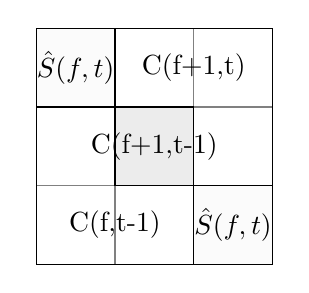
\begin{tikzpicture}
		\draw[step=1cm,color=gray] (0,0) grid (3,3);
		
		\draw[fill=gray!50, fill opacity=0.3] (1,1) -- (1,2) -- (2,2) -- (2,1) -- (1,1);
		\draw[fill=gray!10, fill opacity=0.3] (0,2) -- (0,3) -- (1,3) -- (1,2) -- (0,2);
		\draw[fill=gray!10, fill opacity=0.3] (2,0) -- (3,0) -- (3,1) -- (2,1) -- (2,0);
		
		
		\node[color=black] at (0.5,2.5) {$\hat S(f,t)$};
		\node[color=black] at (2.5,0.5) {$\hat S(f,t)$};
		\node at (1.5,1.5) {C(f+1,t-1)};
		
		
		
		\draw[color=black] (0,0) -- (0,2) -- (2,2) -- (2,0) -- (0,0);
		\draw[color=black] (3,3) -- (1,3) -- (1,1) -- (3,1) -- (3,3);
		
		\node[color=black] at (1,0.5) {C(f,t-1)};
		\node[color=black] at (2,2.5) {C(f+1,t)};
		
		\end{tikzpicture}.
	\end{center} The final cost matrix is normalized by width and incentive bias
\[
C = \hat N \left( \frac{ \tilde C_{ft} }{ t-f+1 }, \Omega \right)
\] for all $t,f \in \tilde C$.
	
	\subsection{Symmetry}	
	
	A common feature on dance music tracks is symmetry, that is to say that for any given track it can be mirrored on itself in time and still look almost the same. 
	
	Let \begin{dmath*}
		\Lambda( f,t,d ) = \left\{ 
		S(f+d-1,f), S(f+d, f+1), S(f+d+1, f+2),\ldots, S(t, t-d-1)
		~ \right\} 
	\end{dmath*}take the diagonal $d$ from track $\hat t= S( i \ge f \le t, j \ge f \le t)$. For each diagonal in $\hat t$ we want to compare each element against its mirror counterpart. `symmetric' pairs that contain the same sign are multiplied together. Pairs that have a different sign are set to $0$ and 
	
	Let symmetry cost matrix
	\begin{dmath*} \frac{1}{t-f+1} \cdot \mathrm{Sym}(f, t, \Omega, \hat \delta) =  
		\sum_{d=1}^{t-f+1} 
		\sum_{i=1}^{|\Lambda( f,t,d )|}{ \left\{
			\begin{array}{lr}
				\mathrm{sign}( \kappa_{i} ) \ne \mathrm{sign}( \rho_i )  & : 0   \\
				\mathrm{sign}( \kappa_{i} ) = \mathrm{sign}( \rho_i ) & : \hat \delta( \kappa_{i}, \rho_i, \Omega )  \\
			\end{array}
			\right.}
	\end{dmath*}  where  $\kappa=\Lambda( f,t,i )$ and $\rho_i = \Lambda( f,t,i )_x$ for $x=|\Lambda( f,t,i )|, |\Lambda( f,t,i )|-1,\ldots,1$.
	
	
	We will consider $3$ types of symmetry cost matrix. The standard symmetry version where 
		\begin{dmath*}\hat \delta( p,q, \Omega ) = \left\{
				\begin{array}{lr}
					\mathrm{sign}(p|q)=-1  & : (1-\Omega) ( p \cdot q ) \\
					\mathrm{sign}(p|q)= 1  & : (\Omega) ( p \cdot q )    \\
				\end{array}
				\right.
		\end{dmath*}
		
		Symmetry summation:
		\begin{dmath*}\hat \delta( p,q, \Omega ) = \left\{
			\begin{array}{lr}
				\mathrm{sign}(p|q)=-1  & : (1-\Omega) \frac{1}{2} ( p + q ) \\
				\mathrm{sign}(p|q)= 1  & : (\Omega) \frac{1}{2} ( p + q )    \\
			\end{array}
			\right.
	\end{dmath*}
	
	The Symmetry change matrix is defined where $\hat \delta$ is the same as the Symmetry summation and the inner sum of the definition becomes the first order differences. For the sake of brevity we have omitted the dynamic programming formulations which run in $O(TW^2)$ time but they have been implemented in code and are available on-line (see Section~\ref{sec:materials}).
	
	\subsection{Evolutionary Contiguity}
	
	\subsection{Static Contiguity}
	
	\subsection{Gaussian}
	Let \[
	G( \varpi, N )_{tw} = e^{ - \frac{1}{2} \frac{\varpi n}{ \frac{1}{2} W}^2  }
	\] for all $n=1,2,\ldots,W$ denote the Gaussian matrix cost function of $N\times W$. $G( \varpi, N )$ is time-independent and every row is the same. We will use this cost function for regularising the others and for use on its own for comparison against a `naive' competitor. Increasing values of $\varpi$ will tighten up the Gaussian although after experimentation we observed that $1$ was always the best value.
	
	\section{Mixing Cost Functions}
	
	We mix cost matrices together by adding them together. In our experiments we will have a parameter for each cost matrix $\biguplus_{\mathrm{costfunction}} \in [0,1]$ to show its contribution to the mixture. The cost matrices will be multiplied by this number before being mixed. 
	
	\section{Computing Best Segmentation}\label{best_cost}
	
	We obtain the cost of a full segmentation by summing the costs of its tracks. The goal is now to efficiently compute the segmentation of least cost.
	
	
	A sequence $\t = (t_1, \ldots, t_{m+1})$ is called an $m/T$-segmentation if
	\[
	1 = t_1 < \ldots < t_m < t_{m+1} = T+1.
	\]
	$m$ is the number of tracks we are trying to find and is a parameter of the algorithm. We use the interpretation that track $i \in \{1, \ldots, m\}$ comprises times $\{t_i, \ldots, t_{i+1}-1\}$. Let $\segs^T_m$ be the set of all $m/T$-segmentations. Note that there is a very large number of possible segmentations 
	\begin{multline*}
		|\segs^T_m| ~=~ \binom{T-1}{m-1}
		= \frac{(T-1)!}{(m-1)!(T-m)!} =\\
		\frac{(T-1)(T-2)\cdots(T-m+1)}{(m-1)!} \ge \left( \frac{T}{m}\right)^{m-1}.
	\end{multline*} 
	For large values of $T$, considering all possible segmentations using brute force is infeasible. For example, a two hour long show with $25$ tracks would have more than $\left( \frac{60^2 \times 2}{25}\right)^{24}  \approx 1.06 \times 10^{59}$ possible segmentations! 
	
	We can reduce this number slightly by imposing upper and lower bounds on the song length.  Recall that $W$ is the upper bound (in seconds) of the song length, $w$ the lower bound (in seconds) and $m$ the number of tracks. With the track length restriction in place, the number of possible segmentations is still massive. A number now on the order of $10^{56}$ for a two hour show with $25$ tracks, $w=190$ and $W=60\times15$.
	
	
	
	Let $N(T,W,w,m)$ be the number of segmentations with time $T$ (in tiles),
	
	We can write the recursive relation $$N(T,W,w,m) = \sum N(t_m-1,W,w,m-1)$$, where the sum is taken over $t_m$ such that 
	\begin{align*}
		t_m &\le T-w+1 & t_m &\ge T-W+1\\
		t_m &\ge (m-1)w+1 & t_m &\le (m-1)W+1
	\end{align*}
	
	The first two inequalities mean that the length of the last track is within an acceptable boundary between $w$ and $W$. The last two inequalities mean that the lengths of the first $m-1$ tracks are within the same boundaries. 
	
	We calculated the value of $N(7000, 60\times15, 190, 25)$ and got $5.20 \times 10^{56}$ which is still infeasible to compute with brute force.
	
	
	
	Our solution to this problem is to find a dynamic programming recursion.
	
	The loss of an $m/T$-segmentation $\t$ is 
	\[
	\loss(\t) 
	~=~
	\sum_{i=1}^m C(t_i, t_{i+1}-1)
	\]
	We want to compute
	\[
	\best^T_m ~=~ \min_{\t \in \segs^T_m} \loss(\t)
	\]
	To this end, we write the recurrence
	\begin{equation*}
		\best^t_1 ~=~ C(1, t) 
	\end{equation*}
	and for $i\ge2$
	\begin{multline*}
		\best^t_i ~=~
		\min_{\t \in \segs^t_i} \loss(\t)
		~=~ \min_{t_i} \min_{\t \in \segs^{t_i-1}_{i-1}} \loss(\t) + C(t_i, t)~=~  \\
		\min_{t_i} C(t_i, t) + \min_{\t \in \segs^{t_i-1}_{i-1}} \loss(\t) 
		~=~ \min_{t_i} C(t_i, t) + \best^{t_i-1}_{i-1}
	\end{multline*}
	%On page 7: t_i should range from t-W to t-w. It is about the position of the /last/ song.
	
	In this formula $t_i$ ranges from $t-W$ to $t-w$. We have $T \times m$ values of $\best^T_m$ and calculating each takes at most $O(W)$ steps. The total time complexity is $O(TWm)$.
	
	\begin{figure*}[t]
		\centering
		%\includegraphics[width=0.45\textwidth]{simmat_preds1.pdf}
		%\hspace{1em}
		\includegraphics[width=\textwidth]{images/simmat_preds}
		
		\caption{An illustration of the similarity matrix $S$ with the reconstructed indexes superimposed. White crosses indicate the human captured indices, and black dotted lines are the reconstructed indices. Note the error where one track has an end segment which is unlike the rest. }
		\label{fig:predictions}
	\end{figure*} 
	
	
	
	
	\section{Posterior Marginal of Song Boundary}
	Fix a learning rate $\eta$, and fix $T$ and $M$. Let
	\[
	P(j,s) ~=~ 
	\frac{\displaystyle
		\sum_{\t \in \segs^T_m : t_j = s} e^{- \eta \loss(\t)}
	}{\displaystyle
	\sum_{\t \in \segs^T_m} e^{- \eta \loss(\t)}
}
\]
That is, $P(j,s)$ is the ``posterior probability'' that song $j$ starts at time $s$.

To compute $P(j,s)$, we need an extended notion of segmentation. We call $\t$ a $m/F: T$ segmentation if
\[
F = t_1 < \ldots < t_m < t_{m+1} = T+1.
\]
Let $\segs^{F : T}_m$ be the set of all $m/F-T$-segmentations. 
%
We have
\begin{multline*}
	\sum_{\t \in \segs^T_m : t_j = s} e^{- \eta \loss(\t)}
	~=~
	\sum_{\substack{\t \in \segs^{s-1}_{j-1},\\ 
			\t'\in \segs^{s : T}_{m-j+1}}} 
	e^{- \eta (\loss(\t) +\loss(\t'))}
	~=~ \\
	\left(\sum_{\t \in \segs^{s-1}_{j-1}} e^{- \eta \loss(\t)}\right)
	\left(\sum_{\t \in \segs^{s : T}_{m-j+1}} e^{- \eta \loss(\t)}\right)
\end{multline*}
%
which upon abbreviating
\begin{align*}
	\head^t_m & ~=~ \sum_{\t \in \segs^{t}_{m}} e^{- \eta \loss(\t)} &
	\tail^f_m & ~=~ \sum_{\t \in \segs^{f : T}_m} e^{- \eta \loss(\t)}
\end{align*}
means that we can write
\[
P(j,s) ~=~ \frac{\head^{s-1}_{j-1} \cdot \tail^{s}_{m-j+1}}{\head^T_m}
.
\]
So it suffices to compute $\head^{t}_{m}$ and $\tail^{t}_{m}$ for all relevant $t$ and $m$. We use
\begin{align*}
	\head^t_1 &~=~ e^{-\eta C(1,t)} &
	\tail^f_1 &~=~ e^{- \eta C(f, T-f+1)}
\end{align*}
and for $m\ge2$
\begin{align*}
	\head^t_m 
	&~=~ 
	\sum_{t_m} \sum_{\t \in \segs^{t_m-1}_{m-1}} e^{- \eta (\loss(\t) + C(t_m, t-t_m+1))} 
	\\
	&~=~ 
	\sum_{t_m} e^{-\eta C(t_m, t-t_m+1)} \sum_{\t \in \segs^{t_m-1}_{m-1}} e^{- \eta \loss(\t)}
	\\
	&~=~ 
	\sum_{t_m} e^{-\eta C(t_m, t-t_m+1)} \head^{t_m-1}_{m-1}
	\\
	\tail^f_m 
	&~=~ 
	\sum_{t_2} \sum_{\t \in \segs^{t_2 : T}_{m-1}} e^{- \eta (C(f, t_2-f)
		+ \loss(\t))}\\
	&~=~
	\sum_{t_2} e^{- \eta C(f, t_2-f)} \sum_{\t \in \segs^{t_2 : T}_{m-1}} e^{- \eta \loss(\t)}\\
	&~=~
	\sum_{t_2} e^{- \eta C(f, t_2-f)} \tail^{t_2}_{m-1}\\
\end{align*}



\section{Posterior Marginal of Song Position}
Fix a learning rate $\eta$, and fix $T$ and $M$. Let
\[
P(j,s,f) ~=~ 
\frac{\displaystyle
	\sum_{\t \in \segs^T_m : t_j = s \land t_{j+1}-1 = f} e^{- \eta \loss(\t)}
}{\displaystyle
\sum_{\t \in \segs^T_m} e^{- \eta \loss(\t)}
}
\]
That is, $P(j,s,f)$ is the ``posterior probability'' that song $j$ starts at time $s$ and finishes at time $f$.
%
In the same vein as the last section, we now get
\[
P(j,s,f) ~=~ \frac{\head^{s-1}_{j-1} \cdot e^{-\eta C(s, f-s+1)} \cdot \tail^{f+1}_{m-j}}{\head^T_m}.
\]

\section{Methodology}

We selected $6$ shows at random (two of each show type) to use to develop the cost matrices and to find an optimal set of parameters using a random search. These shows were A State of Trance $453$ and $462$, Magic Island $98$ and $112$ and Trance Around the World $364$ and $372$.



\section{Materials}\label{sec:materials}

All of the code presented in this paper with the small working test set is available on GitHub \footnote{\url{github.com/ecsplendid/DanceMusicSegmentation}}. The large data set ($\approx100$GB) we received from Dennis Goncharov can easily be made available on request (it is in a Google Drive account).

\section{Results}


\begin{table*}[t]
	\centering
	\begin{tabular}{|llllllll|lll|llllll|}
		\hline 
		
		\begin{sideways}Summation\end{sideways}&\begin{sideways}Symmetry\end{sideways} &\begin{sideways}Evolution\end{sideways}&\begin{sideways}Contig Past\end{sideways} &\begin{sideways}Contig Future\end{sideways}&\begin{sideways}Sym Diff\end{sideways}&\begin{sideways}Sym Sum\end{sideways} &\begin{sideways}Gaussian\end{sideways} &  \begin{sideways}Mean\end{sideways} & \begin{sideways}Heuristic\end{sideways} & \begin{sideways}Shift\end{sideways} & \begin{sideways}60s(\%)\end{sideways} & \begin{sideways}30s(\%)\end{sideways} & \begin{sideways}20s(\%)\end{sideways} & \begin{sideways}10s(\%)\end{sideways} & \begin{sideways}5s(\%)\end{sideways} & \begin{sideways}1s(\%)\end{sideways}    \\ \hline 
		
		
		
		\hline 
	\end{tabular}
	\caption{TODO: place results here}
\end{table*}


\section{Summary}\label{conclusions}

We believe our algorithm would be useful for segmenting DJ-mixed audio streams in batch mode. Our overall average is encouraging, taking into account the difficulty of the task at hand. The similarity matrix we use is based solely on instrument features. 

\textbf{TODO: percussive features}
We captured the percussive features by taking the cross correlation of the samples in the time domain, and using the same convolution filter. 

We would also like to implement some of the methods in the literature (which were mostly designed for scene analysis) to see if we outperform them. It would be tricky to get an exact comparison because we could not find a unsupervised deterministic algorithm which finds a fixed number of strictly contiguous clusters. We could however adapt existing algorithms to get a like for like comparison. We would like to evaluate the performance of J Theiler's contiguous K-means algorithm in particular \cite{theiler1997contiguity} and also similar algorithms. We have the property of being deterministic but probabilistic methods should be explored. Theiler's algorithm would require some modification to work in this scenario because we require strictly contiguous clusters, not just a contiguity bias. 

Another idea would be to add a cost function to account for how many contiguous region transients exist for all potential song placements. 

\section{Acknowledgements}

We would like to thank Mikael Lindgren and Dennis Goncharov from cuenation\footnote{\url{http://www.cuenation.com}} for their help explaining how they make cue sheets and for providing the data set to test the algorithm on.


\bibliographystyle{ieeetr}
\bibliography{bib/references,bib/refs}

\end{document}
